 \begin{figure}
 \centering
 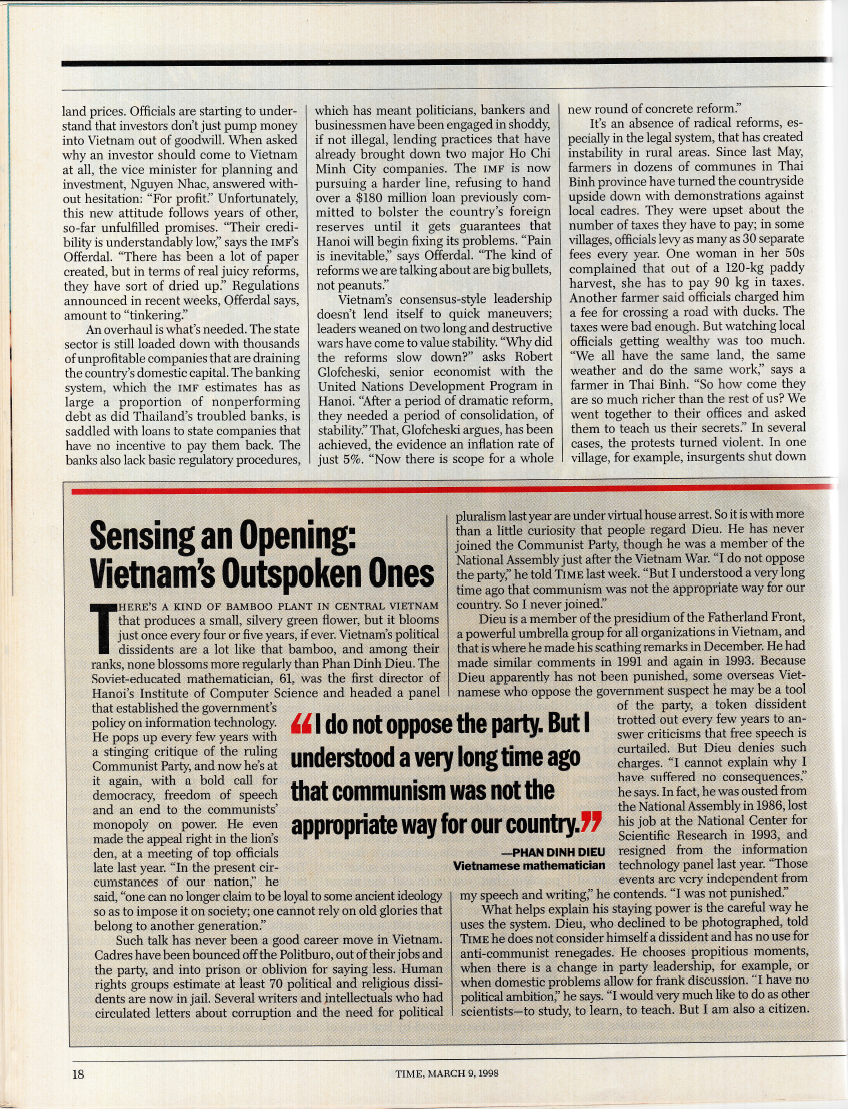
\includegraphics[scale=0.3]{Photos/Time1}
 \end{figure}
 

{\huge  Sensing an Opening: Vietnam’s Outspoken Ones}

\epigraph{I do not oppose the party. But I understood a very long time ago that communism was not the appropriate way for our country.}{\textit{PHAN DINH DIEU – Vietnamese mathematician}}




There’s a kind of bamboo plant in central, Vietnam that produces a small, silvery green flower, but it blooms just once every four or five years, if ever, Vietnam’s political dissidents are a lot like that bamboo, and among their ranks, none blossoms more regularly than Phan Dinh Dieu. The Soviet-educated mathematician, 61, was the first director of Hanoi’s Institute of Computer Science and headed a panel that established the gorvernment’s policy on information technology. He pops up every few years with a stinging critique of ruling Communist Party, and now he’s at it again, with a bold call for democracy, freedom of speech and an end to the communists’ monopoly on power,. He even made the appeal right in the lion’s den, at a meeting of top officials late last year. “In the present circumstances of our nation,” he said, “one can no longer claim to be loyal to some ancient ideology so as to impose it on society; one cannot rely on old glories that belong to another generation.”

 Such talk has never been a good career move in Vietnam. Cadres have been bounced off the Politburo, out of their jobs and the party, and into prison or oblivion for saying less. Human rights groups estimate at least 70 political and religious dissidents are now in jail. Several writers and intellectuals who had circulated letters about corruption and the need for political pluralism last year are under virtual house arrest. So it is with more than a little curiosity that people regard Dieu. He has never joined the Communist Party, though he was a member of the National Assembly just after the Vietnam War. “I do not oppose the party,” he told TIME last week. “But I understood a very long time ago that communism was not the appropriate way for our country. So I never joined.”
 
 Dieu is a member of presidium of Fatherland Front, a powerful umbrella group for all organizations in Vietnam, and that is where he made his scathing remarks in December. He had made similar comments in 1991 and again in 1993. Because Dieu apparently has not been punished, some overseas Vietnamese who oppose the government suspect he may be a tool of the party, a token dissident trotted out every few years to answer criticisms that free speech is curtailed. But Dieu denies such charges. “I cannot explain why I have suffered no consequences,” he says. In fact, he was ousted from the National Assembly in 1986, lost his job at the National Center for Scientific Research in 1993, and resigned from the information technology panel last year. “Those events are very independent from my speech and writing,” he contends. “I was not punished.”
 
 What helps explain his staying power is the careful way he uses the system. Dieu, who declined to be photographed, told TIME he does not consider himself a dissident and has no use for anti-communist renegades. He chooses propitious moments, when there is a change in party leadership, for example, or when domestic problems allow for frank discussion. “I have no political ambition,” he says. “I would very much like to do as other scientists – to study, to learn, to teach. But I am also a citizen. I have to contribute to the life of our country.”
 
A confluence of events-rural unrest in Thai Binh province, an economic downturn and the installation last year of a new leadership-seems to have inspired others, like Dieu, to express their dissent. A retired general, Tran Do, wrote an open letter to party leaders, warning, “If we do not kick our-selves out of this sickly morass we will collapse…and if we let the morass linger on, then we will have increasing social instability.” In a letter to the party leadership, Hoang Huu Nhan, a former high-ranking economics adviser to the party, has called for more dramatic economic reforms. “People seem to be emboldened,” says Carlyle Thayer, an Australian scholar of Vietnamese politics. “It’s a time of fluidity, and that’s a time for people to get ideas out.” Dieu insists he has not been in communication with Tran Do or Nhan. Thayer suspects, however, that “there are probably many people who agree with him and who invited him to say what they don’t want to be identified with themselves.”

In recent years, the door has sometimes opened a crack to allow such debate, but then closed just as quickly. In the late 1980s, political discourse was relaxed-until Vietnamese leaders saw communist government toppling in Eastern Europe. Dieu and others spoke out during a 1991 leadership change. This time, the new Party General Secretary, Le Kha Phieu, has met with Tran Do and with dissident Hoang Minh Chinh, who has been in and out of prison since the 1960s, according to sources close to the two men. None of these meetings, or speeches like Dieu’s, are publicized in Vietnam’s state-run media, and some prominent writers and journalists have been warned by police not to have contact with Tran Do or Dieu. But the Foreign Ministry, in a written response to questions from foreign journalists, says such criticisms of the party are merely “a normal thing.” A septuagenarian writer is cheered that so far the government hasn’t been responding as it normally does, by cracking down on dissidents. “For 40 years, I have lived on the fringes of society,” he say. But still I have hope. Our current crisis means not all of the leaders can be deaf. Before, they would have thrown this stuff in a trash bin and disciplined the authors. Now, the leave them alone.”

 Many younger Vietnamese are less sanguine. “The party views these people like mosquitoes,” says a writer in his 30s whose bleak portrayals of a disintegrating society have irritated authorities. “They annoy you, but they can’t kill you.” What remains to be seen is whether the vocal dissenters will suffer the same fate as the rarely blooming bamboo plant: after it flowers, it usually dies. Dieu, however, is a survivor. “If I can say what I believe,” he says, “then other people can voice their opinions too, and maybe we can have the beginning of democracy.”
-By Tim Larimer/Hanoi

\newpage

%\chapter*{Báo TIME 1998} \index{Báo chí}
 \begin{figure}
 \centering
 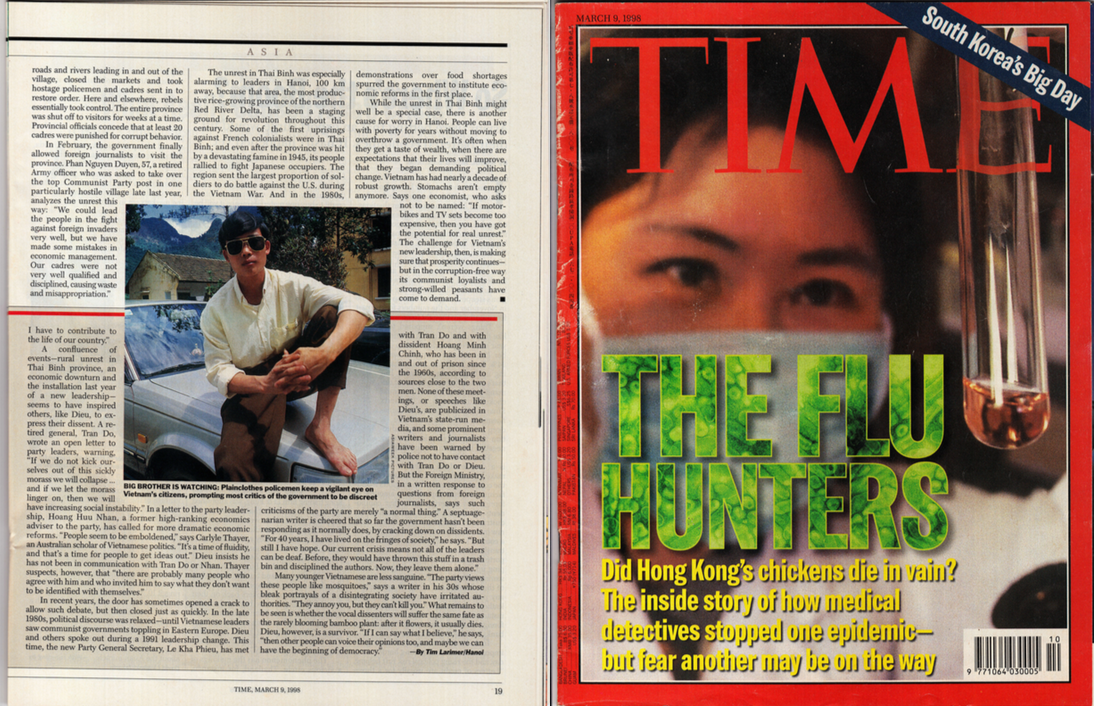
\includegraphics[scale=0.3]{Photos/Time2}
 \end{figure}
 
{\huge Cảm nhận một bước mở cửa: Những người nói thẳng ở Việt Nam}

\epigraph{Tôi không chống Đảng. Nhưng đã từ rất lâu tôi hiểu rằng chủ nghĩa cộng sản không phải là con đường thích hợp với đất nước tôi.}{\textit{PHAN ĐÌNH DIỆU - Nhà Toán học Việt nam }}




    Có một loại cây tre mọc ở miền Trung Việt nam nở một thứ hoa màu xanh ánh bạc rất bé, nhưng có nở thì cũng khoảng bốn năm năm mới nở một lần. Những nhân vật ly khai chính trị của Việt nam khá giống như loài tre đó và trong số họ, không ai trổ hoa đều đặn hơn ông Phan Đình Diệu. Nhà toán học từng học ở Liên Xô, 61 tuổi, ông ta là Viện trưởng đầu tiên của Viện Tin học Hà Nội và đứng đầu một nhóm soạn thảo chính sách của Chính phủ về Công nghệ thông tin. Cứ mỗi vài năm ông ta lại bất ngờ xuất hiện với một sự phê phán sắc bén đối với Đảng Cộng sản cầm quyền, và lần này lại xuất hiện với một lời kêu gọi đậm nét hơn cho dân chủ, tự do ngôn luận, và chấm dứt sự độc tài cộng sản ở chính quyền. Ông ta đưa ra lời kêu gọi đó ngay trong hang sư tử, tại một cuộc họp của nhiều quan chức cao cấp vào cuối năm ngoái . ‘‘Trong điều kiện nước ta hiện nay”, ông ta nói “không thể tiếp tục vin vào lý do trung thành để áp đặt một ý thức hệ lỗi thời cho xã hội, không thể dựa mãi vào những vinh quang dĩ vãng của một thế hệ đi trước”.
    
    Kiểu nói như vậy chưa bao giờ đưa tới một sự nghiệp thăng tiến ở Việt Nam. Có những cán bộ đã bị đưa ra khỏi Bộ Chính trị, bị tước chức vụ và bị khai trừ khỏi Đảng, bị đưa vào tù hoặc vào sự quên lãng để ít nói hơn. Các nhóm nhân quyền đánh giá có ít nhất 70 nhân vật ly khai chính trị và tôn giáo hiện đang bị cầm tù. Một số nhà văn và tri thức phân phát kiểu chuyển tay các bức thư về tham nhũng và yêu cầu đa nguyên chính trị năm ngoái bị quản thúc tại nhà. Chính vì thế mà với ít nhiều tò mò người ta nhìn vào ông Diệu. Ông ta chưa bao giờ vào Đảng Cộng sản, mặc dầu đã là đại biểu Quốc hội ngay sau cuộc chiến tranh Việt nam. “Tôi không chống Đảng”, ông ta nói với TIME tuần trước, “nhưng đã từ rất lâu tôi hiểu rằng chủ nghĩa cộng sản không phải là con đường thích hợp với đất nước tôi. Vì vậy mà không bao giờ tôi vào Đảng”.
    
    Diệu là một ủy viên đoàn chủ tịch Mặt trận Tổ quốc, một hình thức bao trùm lên tất cả các tổ chức ở Việt nam, và đây là nơi mà ông ta đưa ra những lời phê phán gay gắt hồi tháng Chạp vừa qua. Ông ta đã làm những phê bình tương tự vào năm 1991 và lại tiếp tục năm 1993. Vì ông Diệu chưa bị trừng phạt một cách công khai, nên một số người Việt hải ngoại chống chính phủ ngờ rằng ông ta có thể là một công cụ của Đảng, một kẻ ly khai giả mạo, cứ vài năm lại tung ra một lần để trả lời lại những phê phán cho là ngôn luận tự do bi bóp nghẹt. Nhưng ông Diệu bác bỏ những lời buộc tội đó. “Tôi không thể giải thích tại sao tôi chưa phải chịu các hậu quả”, ông ta nói. Thực tế, ông ta đã bị loại ra khỏi quốc hội năm 1981, bị mất chức ở Viện Khoa học Việt  nam 1993, và đã từ chức khỏi Ban Chỉ đạo Quốc gia về công nghệ thông tin năm ngoái. Nhưng ông ta khẳng định: “Những việc đó là hoàn toàn độc lập với những lời nói và bài viết của tôi. Tôi chưa bị trừng phạt”.
    
    Điều giúp ta giải thích cái khả năng bền bỉ của ông ta là ở cái cách thận trọng mà ông ta sử dụng hệ thống. Ông Diệu đã khước từ cho chụp ảnh và nói với TIME rằng ông ta không xem mình là một nhân vật ly khai và không để bị lợi dụng bởi những những người phản kháng chống cộng. Ông ta chọn những thời điểm thuận lợi, khi có một sự thay đổi trong lãnh đạo Đảng chẳng hạn, hay khi những vấn đề trong nước cho phép được thảo luận thẳng thắn. “Tôi không có tham vọng chính trị”, ông ta nói. “Tôi rất muốn được làm như những nhà khoa học khác – nghiên cứu, học tập, giảng dạy. Nhưng tôi cũng là một công dân. Tôi có trách nhiệm đóng góp vào đời sống của đất nước tôi”.

Hàng loạt các sự kiện bất ổn ở vùng nông thôn thuộc tỉnh Thái Bình, kinh tế suy thoái và việc một nhà lãnh đạo nhậm chức đã khiến nhiều người quan tâm như giáo sư Diệu – người đã bày tỏ ý kiến bất đồng. Một tướng quân đội đã nghỉ hưu - ông Trần Độ đã viết thư ngỏ gửi các nhà lãnh đạo Đảng cộng sản, ông cảnh báo: "Nếu chúng ta không tự mình thoát khỏi lý luận giáo điều này chúng ta sẽ sụp đổ và nếu chúng ta cứ để cho lý luận ngày càng bùng nhùng hơn chúng ta sẽ phải chứng kiến những bất ổn xã hội”. Trong một bức thư gửi Lãnh đạo Đảng, ông Hoàng Hữu Nhân – nguyên cố vấn kinh tế cao cấp của Đảng - đã kêu gọi cải cách kinh tế mạnh mẽ hơn nữa. Học giả người Úc nghiên cứu chính trường Việt Nam – ông Carlyle Thayer nói: "Dường như mọi người đã mạnh dạn hơn”. "Đã đến lúc thông thoáng hơn và là lúc để người ta đưa ra quan điểm của mình”. Giáo sư Diệu khẳng định ông không có bất kỳ liên hệ nào với ông Trần Độ và ông Hoàng Nhân. Tuy nhiên, ông Thayer nghi ngờ khi cho rằng: “có thể có nhiều người đồng ý với ông Diệu đã mời ông Diệu phát biểu về những vấn đề mà họ không muốn bị coi là chính họ nêu lên”. 

Trong những năm gần đây, đôi khi cũng có những lúc cởi mở để trao đổi những vấn đề gây tranh cãi nhưng sau đó mọi chuyện khép lại chóng vánh. Cuối những năm 1980, thảo luận chính trị được cởi mở hơn khi các vị lãnh đạo Việt Nam đã chứng kiến chính quyền cộng sản bị lật đổ ở Đông Âu. Giáo sư Diệu và một số người khác đã lên tiếng trong suốt giai đoạn diễn ra thay đổi lãnh đạo năm 1991. Theo một nguồn tin thân cận của hai vị, lần này, tân Tổng Bí thư Lê Khả Phiêu đã gặp tướng Trần Độ và nhà bất đồng chính kiến Hoàng Minh Chính – người mà bị vào tù rồi ra tù suốt những năm 60 -  thông tin về những cuộc gặp hay những phát ngôn của giáo sư Diệu đều không được đăng tải trên các báo chính thống. Một số tay bút kỳ cựu và nhà báo đều được công an Việt Nam cảnh báo không được liên hệ với ông Trần Độ hoặc giáo sư Diệu. Riêng Bộ Ngoại Giao Việt Nam, trong một văn bản trả lời các câu hỏi của các phóng viên nước ngoài nêu những phản biện như vậy đối với Đảng cộng sản đều là những điều “rất bình thường”. Một nhà văn già nói rằng chính phủ Việt Nam không phản ứng như cách thông thường họ làm mà bằng việc đàn áp các nhà bất đồng chính kiến. Ông nói: "Tôi đã sống bên lề xã hội Việt Nam suốt 40 năm nhưng tôi luôn hy vọng. Cơn khủng hoảng hiện nay không có nghĩa mọi nhà Lãnh đạo đều mũ ni che tai. Trước đó, họ đã ném thứ này vào thùng rác và kỷ luật các tác giả. Nhưng bây giờ họ cô lập họ”.

Nhiều thanh niên người Việt không mấy lạc quan cho lắm. Một nhà văn chừng 30 tuổi – người đã có những miêu tả về sự ảm đạm của một xã hội đã khiến các nhà chức trách khó chịu - nói: "Đảng cộng sản luôn coi những người này là những con muỗi. Họ có thể làm phiền anh nhưng không thể giết được anh”. Điều gì còn lại để nhận ra là liệu các nhà bất đồng chính kiến có phải chịu số phận giống cây tre khi sinh sản: sau khi hoa tre nở cây thường chết. Tuy nhiên, giáo sư Diệu là một người sống sót. Ông nói: “Nếu tôi nói điều tôi tin thì người khác cũng có quyền cất lên tiếng nói của mình và đó có thể là sự khởi đầu của một nền dân chủ”.

-By Tim Larimer/Hanoi

